\newpage
\appendix

\section{Dataset Process Details}\label{app_data}

\textbf{Dataset Sources.} Table~\ref{table:video_source_full} provides the full dataset references for the training data summarized in Table~\ref{table:video_source}.

\begin{table}[H]
    \centering
    \small
    \setlength{\tabcolsep}{4pt}
    \renewcommand{\arraystretch}{1}
    \begin{tabularx}{\linewidth}{@{}llX@{}}
        \toprule
        Data Type & Embodiment Type & Data Sources \\
        \midrule
        \multirow{3}{*}{Robot}
        & Single-arm
        & OXE~\citep{collaboration2023openx}, RoboMIND~\citep{wu2025robomind}, DROID~\citep{khazatsky2024droid}, RH20T~\citep{fang2024rh20t}, MolmoAct~\citep{lee2025molmoact} \\
        & Dual-arm
        & AgiBot World-Beta~\citep{bu2025agibot}, RoboCOIN~\citep{wu2025robocoin}, RDT~\citep{liu2024rdt}, GM-100~\citep{wang2026gm100}, ABC-130K~\citep{allshire2026abc}, Self-collected ALOHA Data\\
        & Mobile \& humanoid
        & InternData-A1~\citep{tian2025interndata}, Galaxea Open-World~\citep{jiang2025galaxea}, Self-collected dexterous hands \\
        \midrule
        \multirow{2}{*}{Human}
        & \multirow{2}{*}{Human hands}
        & Open-source: EgoDex~\citep{hoque2025egodex}, Ego4D~\citep{grauman2022ego4d}, EPIC-KITCHENS~\citep{damen2018epic}, Something-Something V2~\citep{goyal2017something,mahdisoltani2018granularity}, VITRA-1M~\citep{li2025vitra} \\
        & & Self-collected egocentric data\\
        \midrule
        General Video
        & Human hands
        & OpenVid~\citep{nan2025openvid}, Panda-70M~\citep{chen2024panda} \\
        \bottomrule
    \end{tabularx}
    \caption{Training data sources with references to the original datasets. Self-collected datasets are collected as part of this work.}
    \label{table:video_source_full}
\end{table}

\subsection{Video Captioning.}\label{app_video}
After segmentation, we use a VLM to generate detailed captions for each clip according to a predefined template. Our captioning pipeline aims to reduce uncertainty in future prediction and encourage consistent mappings from semantic descriptions to visual trajectories. Specifically, we address four major sources of uncertainty:

\textit{(1) Detailed Task Description.}
We describe how the end effector completes the task, including the sequence and manner of manipulation.

\textit{(2) Explicit End-Effector Identification.}
The active end effector must be visible in the first frame; otherwise, we trim the clip to begin when it first becomes visible. When multiple end effectors are involved, we describe the motion of each one explicitly.

\textit{(3) Unambiguous Target-Object Specification.}
When multiple identical or similar objects are present, we identify the target using distinctive attributes or spatial relationships. The target object must also be visible in the first frame.

\textit{(4) Camera-View Description.}
We use optical flow to remove egocentric clips with excessive viewpoint changes. For clips with moderate camera motion, a VLM describes the viewpoint changes and the camera views included in the video, and we incorporate this information into the caption.

\subsection{Unified Action Space}

We focus on egocentric bimanual datasets, including ALOHA-style,
humanoid-style, and human egocentric datasets. These datasets
account for more than \(80\%\) of the total data and share a
similar bimanual structure and camera viewpoint.
We explicitly align their coordinate systems at two levels:
(1) \textit{workspace alignment}, which applies a world-frame
transformation so that different robots have comparable
end-effector workspaces; and (2) \textit{end-effector alignment},
which applies a local transformation to standardize end-effector
origins and axis orientations. 

% Such alignment is necessary because different datasets adopt different end-effector conventions. For example, some place the eef origin between the fingertips, whereas others place it at the gripper mounting link. Similarly, some align the \(x\)-axis with the gripper direction, while others define it perpendicular to that direction.

For an arm dataset \(d\) , let
\(T_d = {}^{W_d}T_{E_d} \in SE(3)\) denote the original
end-effector pose, where \(W_d\) and \(E_d\) are the dataset's
world and end-effector frames, respectively.
We define the workspace alignment as
\(A_d = {}^{\bar{W}}T_{W_d}\) and the end-effector alignment as
\(B_d = {}^{E_d}T_{\bar{E}}\), where \(\bar{W}\) and \(\bar{E}\)
denote the canonical world and end-effector frames.
The aligned end-effector pose is given by
\begin{equation}
    \widetilde{T}_d = A_d T_d B_d,
    \label{eq:coordinate_alignment}
\end{equation}
% where \(A_d \in SE(3)\) aligns the world coordinate system
% through left multiplication, and \(B_d \in SE(3)\) aligns
% the end-effector origin and axis orientations through
% right multiplication.
% Such alignment is necessary because different datasets adopt
% different end-effector conventions. For example, some place
% the end-effector origin between the fingertips, whereas others
% place it at the gripper mounting link. Similarly, some align
% the \(x\)-axis with the gripper direction, while others define
% it perpendicular to that direction. The local transformation
% \(B_d\) accounts for both the origin offset and the difference
% in axis orientations.
\newpage
\section{More Video Prediction Results}
% Additional video prediction results on open-ended tasks. We compare single-step video predictions before and after distillation. Distillation enables high-quality video prediction with just one sampling step, as shown in Figure~\ref{fig:video_app}.


\begin{figure}[h]
    \centering
    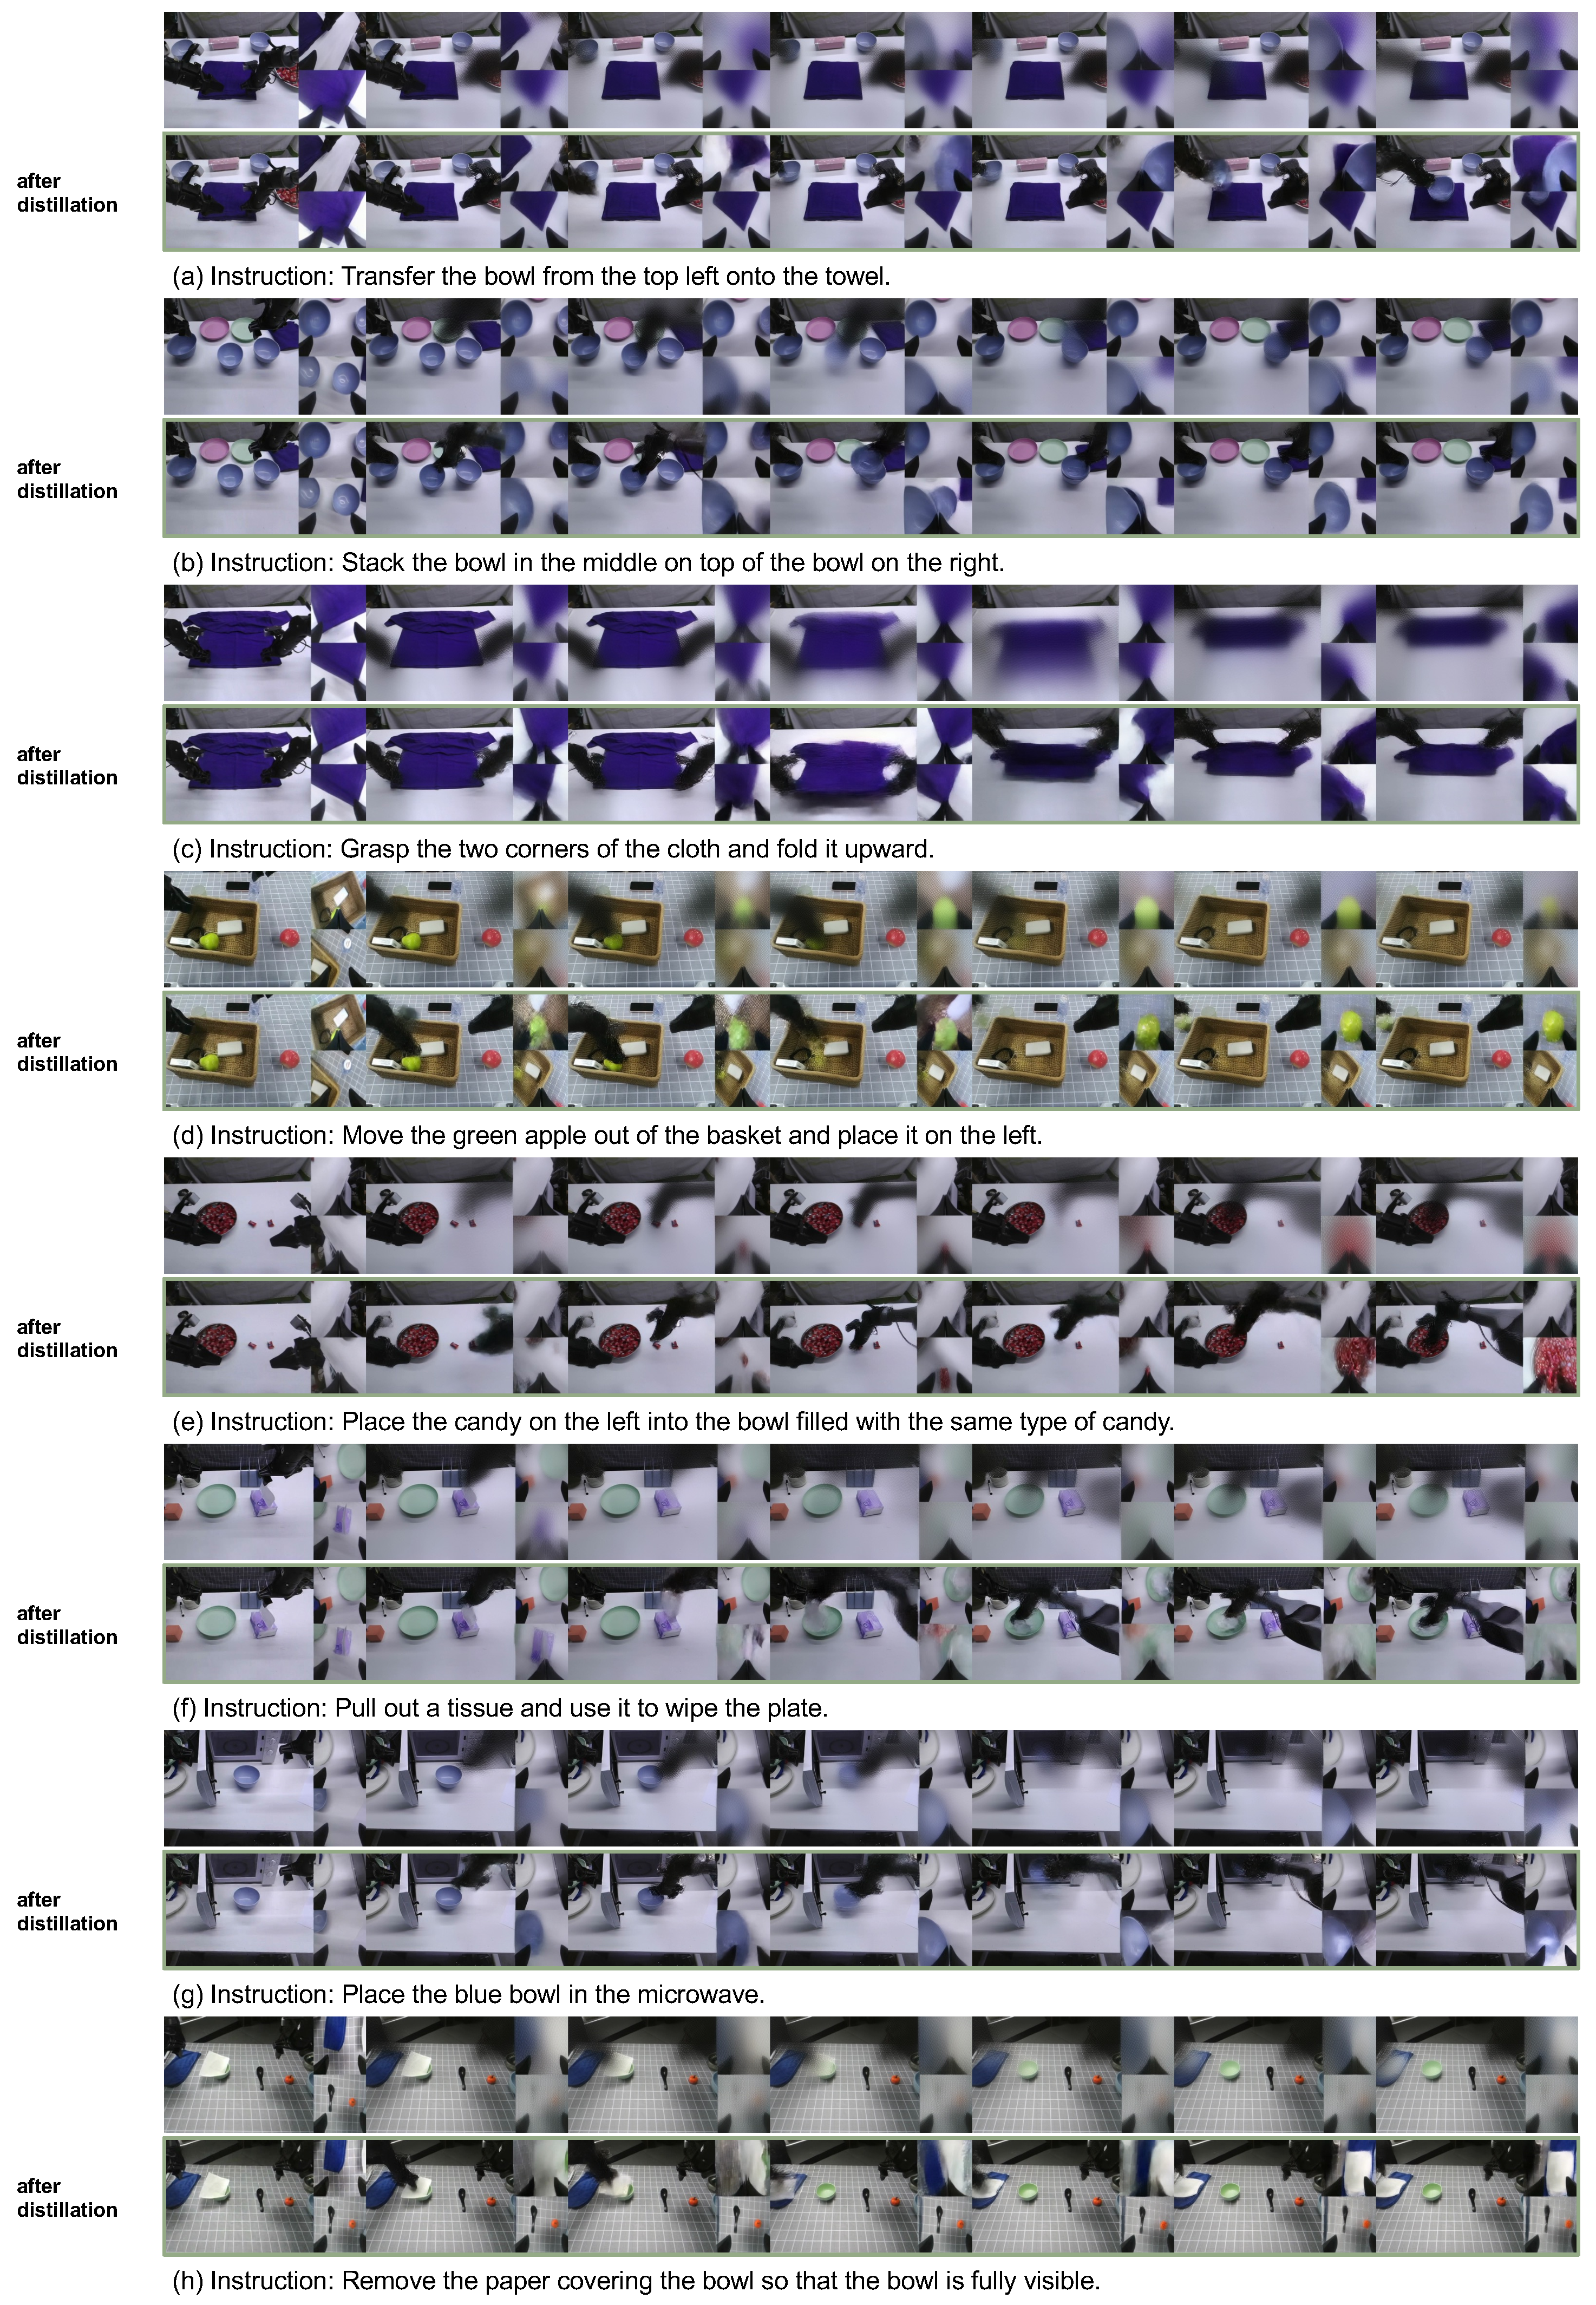
\includegraphics[width=0.96\linewidth]{figures/video_comparison_8groups_updated.pdf}
    \caption{Additional video prediction results on open-ended tasks. We compare \textbf{single-step} video predictions before and after distillation. Distillation enables high-quality video prediction with just one sampling step.}
    \label{fig:video_app}
\end{figure}

\newpage
\section{Detailed Benchmark Results}\label{app_results}
\subsection{Detailed LIBERO Results}\label{app_libero}
Table~\ref{tab:app_libero} reports per-suite success rates on the four standard LIBERO suites~\citep{liu2023libero}, which correspond to the LIBERO-ID results in Table~\ref{tab:libero_generalization}. Baseline results are taken from the original papers and from \citet{zhang2026harness} and \citet{mishra2026understanding}.

\begin{table}[h]
\centering
\small
\begin{tabular}{lccccc}
\toprule
Method & Spatial & Object & Goal & Long & Avg. \\
\midrule
$\pi_0$~\citep{black2024pi_0} & 96.8 & 98.8 & 95.8 & 85.2 & 94.2 \\
$\pi_{0.5}$~\citep{intelligence2025pi_} & 98.8 & 98.2 & 98.0 & 92.4 & 96.9 \\
MolmoAct~\citep{lee2025molmoact} & 87.0 & 95.4 & 87.6 & 77.2 & 86.6 \\
X-VLA~\citep{zheng2026xvla} & 98.2 & 98.6 & 97.8 & 97.6 & 98.1 \\
AtomVLA~\citep{sun2026atomvla} & 96.4 & 99.6 & 97.6 & 94.4 & 97.0 \\
\midrule
Cosmos-Policy~\citep{kim2026cosmospolicy} & 98.1 & \textbf{100.0} & 98.2 & 97.6 & 98.5 \\
Fast-WAM~\citep{yuan2026fastwam} & 98.2 & \textbf{100.0} & 97.0 & 95.2 & 97.6 \\
DiT4DiT~\citep{ma2026dit4dit} & 98.4 & 99.6 & \textbf{98.6} & 97.6 & 98.6 \\
Temporal Ratio~\citep{mishra2026understanding} & 96.3 & 99.6 & 97.6 & 82.6 & 94.0 \\
\midrule
\textbf{VPP2 (Ours)} & \textbf{99.2} & 99.8 & 98.2 & \textbf{98.0} & \textbf{98.8} \\
\bottomrule
\end{tabular}
\caption{Per-suite success rates (\%) on the standard LIBERO benchmark. Best results in each column are in bold.}
\label{tab:app_libero}
\end{table}

\subsection{Detailed RoboDojo Results}\label{app_robodojo}
RoboDojo~\citep{chen2026robodojo} evaluates generalist manipulation policies on 42 bimanual simulation tasks organized into five capability dimensions. \textit{Generalization} tests robustness to unseen backgrounds, lighting, clutter, and target objects, and is evaluated under both standard and randomized settings. \textit{Precision} requires fine-grained target localization and contact-rich control. \textit{Long-Horizon} requires completing all sub-steps of multi-step tasks. \textit{Memory} contains tasks whose correct actions depend on information observed earlier in the episode. \textit{Open} evaluates unseen task specifications whose required skills appear in the training data under different contexts. We follow the official training and evaluation protocol. The average score captures partial task progress, and the success rate measures binary task completion.

Tables~\ref{tab:app_robodojo_score} and~\ref{tab:app_robodojo_sr} report the per-dimension average score and success rate, respectively, complementing Table~\ref{tab:robodojo}. Baseline results are taken from the official RoboDojo simulation leaderboard as of September 2026.

\begin{table}[h]
\centering
\small
\setlength{\tabcolsep}{3.5pt}
\begin{tabular}{lccccccc}
\toprule
 & \multicolumn{2}{c}{Generalization} & & & & & \\
\cmidrule(lr){2-3}
Method & Std. & Rand. & Precision & Long-Horizon & Memory & Open & Avg. \\
\midrule
$\pi_0$~\citep{black2024pi_0} & 7.18 & 0.71 & 3.56 & 6.19 & 3.47 & 0.25 & 3.48 \\
$\pi_{0.5}$~\citep{intelligence2025pi_} & 20.93 & 5.82 & 12.40 & 23.54 & 5.89 & 1.98 & 11.44 \\
X-VLA~\citep{zheng2026xvla} & 17.90 & 3.04 & 18.32 & 16.53 & 4.76 & 0.55 & 10.13 \\
Fast-WAM~\citep{yuan2026fastwam} & 4.33 & 0.34 & 1.96 & 9.14 & 3.55 & 0.42 & 3.48 \\
OpenWAM-$\alpha$~\citep{wang2026openwam} & 33.16 & 8.26 & 18.45 & 34.93 & 10.41 & 1.41 & 17.18 \\
Xiaomi-Robotics-1~\citep{guo2026xiaomirobotics1} & 35.65 & 11.44 & 26.69 & 38.39 & 7.81 & 3.94 & 20.07 \\
GPT-6-Astra~\citep{zhang2026astra} & 35.32 & 31.40 & 12.65 & 21.45 & 43.04 & 34.36 & 28.97 \\
\midrule
\textbf{VPP2 (Ours)} & \multicolumn{2}{c}{36.39} & 43.03 & 56.28 & 56.01 & 4.61 & \textbf{39.26} \\
\bottomrule
\end{tabular}
\caption{Per-dimension average score on the RoboDojo simulation benchmark. Generalization is evaluated under standard (Std.) and randomized (Rand.) settings. Avg.\ is the mean over the five capability dimensions, where the generalization score is the mean of the Std.\ and Rand.\ settings. For VPP2, we report the generalization result pooled over both settings (25 episodes each, following the official protocol), which equals their mean. Baseline results are taken from the official leaderboard.}
\label{tab:app_robodojo_score}
\end{table}

\begin{table}[t]
\centering
\small
\setlength{\tabcolsep}{3.5pt}
\begin{tabular}{lccccccc}
\toprule
 & \multicolumn{2}{c}{Generalization} & & & & & \\
\cmidrule(lr){2-3}
Method & Std. & Rand. & Precision & Long-Horizon & Memory & Open & Avg. \\
\midrule
$\pi_0$~\citep{black2024pi_0} & 4.89 & 0.22 & 0.75 & 2.00 & 2.11 & 0.25 & 1.53 \\
$\pi_{0.5}$~\citep{intelligence2025pi_} & 14.89 & 1.44 & 5.50 & 14.67 & 4.67 & 1.67 & 6.93 \\
X-VLA~\citep{zheng2026xvla} & 12.22 & 1.33 & 12.00 & 9.75 & 3.56 & 0.50 & 6.52 \\
Fast-WAM~\citep{yuan2026fastwam} & 2.11 & 0.11 & 0.00 & 5.17 & 3.44 & 0.42 & 2.03 \\
OpenWAM-$\alpha$~\citep{wang2026openwam} & 25.56 & 4.11 & 9.25 & 25.33 & 9.11 & 1.08 & 11.92 \\
Xiaomi-Robotics-1~\citep{guo2026xiaomirobotics1} & 28.00 & 6.00 & 18.83 & 23.67 & 6.56 & 3.58 & 13.93 \\
GPT-6-Astra~\citep{zhang2026astra} & 32.67 & 28.33 & 4.00 & 8.25 & 38.67 & 31.00 & 22.48 \\
\midrule
\textbf{VPP2 (Ours)} & \multicolumn{2}{c}{29.50} & 35.17 & 37.00 & 55.56 & 4.08 & \textbf{32.26} \\
\bottomrule
\end{tabular}
\caption{Per-dimension success rate (\%) on the RoboDojo simulation benchmark, computed in the same way as Table~\ref{tab:app_robodojo_score}.}
\label{tab:app_robodojo_sr}
\end{table}
